\chapter*{Комбинаторика}

\epigraph{Ложь имеет бесконечное число комбинаций,\\
тогда как правда бывает только одна.}{Жан-Жак Руссо}


                                                                             
                                                        
Если задача начинается со слов  «Сколько существует способов...», то это автоматически задача комбинаторная, хотя обратное неверно.   Комбинаторный подход 
будет нам полезен при решении нижеследующих (достаточно эклектичных%???довольно разнообразных
) задач и многих других в этой книге.   


Наша показательная задача совершенно классическая и использует фундаментальную
комбинаторную технику  --- перемножение числа%???
возможных вариантов.   




\subsection*{Расстановка цифр}% (Sequencing the Digits)


Сколькими способами можно записать в ряд цифры от 0 до 9, так, что каждая цифра, кроме самой левой, отличается от одной из цифр стоящих слева от неё, на единицу.%???подправил


\paragraph{Решение:} На первый взгляд кажется, что данная задача не решается  при помощи  перемножения числа %???
возможных вариантов, так как количество вариантов зависит от предыдущего выбора.
Например, мы имеем %???у нас есть
десять вариантов для самой левой цифры,
но начав ряд, скажем,  с «3» у нас только два варианта для следующей цифры; если же мы начинаем с «0» или  «9», то у нас только один выбор. Если вы знакомы с суммированием биноминальных коэффициентов, вы можете проанализировать таким образом решение задачи, но рассмотрим лучший способ. %???


Заметим, что последовательность обрывается %???заканчивается нулём или девяткой
«0» или «9»; и %???
если мы \emph{движемся справа налево}, мы всегда  %???каждый раз
стоим перед выбором --- написать наибольшую неиспользованную цифру или наименьшую, пока не дойдём до левого края, где эти два выбора совпадают.
Таким образом, мы получаем два выбора в каждой из девяти возможностей.
Следовательно%???отсюда
, конечный ответ $2^9=512$ способов.\heart


(Источник:   Олимпиада Патнема 1960-х годов%  (A Putman Exam from the 1960s )
%???Другие решения можно найти в статье ...
)


За вами решение оставшихся задач.
Подсказка: смотрите внимательно, где можно применить принцип Дирихле!








\subsection*{Подмножества подмножеств}% (Subsets of subsets)


Докажите, что любое множество из десяти различных чисел от 1 до 100 содержит два непересекающихся непустых подмножества, сумма чисел которых одинакова.


\subsection*{Вредный метрдотель}%  (The Malicious Maitr D’)


На банкете математической конференции 48-ми  мужчинам математикам, ни один из которых не имеет ни малейшего представления об этикете, назначены места за большим круглым столом. На столе, между каждой парой приборов, стоит кофейная чашка с салфеткой.
Как только человек занимает своё место (по указанию метрдотеля), он берёт салфетку, слева или справа от себя; если на столе две салфетки, он выбирает одну случайным образом (но метрдотель не должен видеть, какую ).

%В каком порядке следует заплнять места???
В каком порядке должны заполняться места, чтобы максимальному количеству математиков  %(maximize the expected number) 
не досталось салфетки?




\subsection*{Рукопожатия на приёме}% (Handshakes at a Party)


Майк и Жанна, а также ещё четыре пары, побывали на праздничном обеде, где каждый из присутствующих обменялся рукопожатием с каждым ему дотоле незнакомым гостем. Позже Майк опросил всех и обнаружил, что каждый из девяти других  гостей пожал руки с различным количеством человек. 


  Со сколькими гостями обменялась рукопожатиями Жанна?




\subsection*{Трёхсторонние выборы}%    (Three-Way Election)


Ашворд%???Ашфорд
, Бакстер и Кэмпбелл баллотируются на пост председателя  союза %(secretary of union) 
и набирают  по одинаковому количеству голосов. Для разрешения этой ситуации они требуют голосования с учётом второго выбора избирателей (т. н. преференциального метода голосования), но снова приходят к ничьей.  Тогда Ашворд выступает с предложением, что, так как количество избирателей нечётное,  можно провести двухсторонние выборы  --- избиратели выбирают между  Бакстером и Кэмпбеллом, а затем между победителем и Ашвордом.


Но Бакстер недоволен данным предложением. Он считает этот способ несправедливым, потому что, по его мнению, у Ашворда  больше шансов выиграть, чем у остальных. Прав ли Бакстер?


\subsection*{Зарплата короля}% (King’s Salary)%???коровевская зарплата


После революции каждый из 66 жителей некой страны, включая короля, получает зарплату в 1 доллар.
Король не может больше голосовать,  но  всё ещё сохраняет за собой право вносить изменения в законопроект,  в частности,  в то,  как распределяется зарплата.
Зарплата каждого жителя должна быть целым числом долларов и сумма всех зарплат  равняется 66.
Каждое предложение по изменению ставится на голосование и принимается, если получает больше голосов «За», чем «Против».
Будем считать, что те, кто получают прибавку к зарплате, голосуют «За», а те, у кого зарплата уменьшается --- «Против»,  остальные же голосованием себя не утруждают.


Король --- человек умный и корыстный. Какой  максимальной для себя зарплаты он может добиться и сколько шагов ему на это понадобиться?%???потребуется




\subsection*{Плохо сделанные часы}%  (A Poorly Designed Clock)


Есть часы, у которых минутная стрелка никак не отличается от часовой. Сколько раз в день возникнет ситуация, когда  по этим часам нельзя будет определить, сколько времени в данный момент?


          


\subsection*{Таинственный карточный фокус}% (A Mystifying Card Trick ) %???загадочный


Давид и Дороти придумали хитрый карточный фокус. Давид отворачивается, кто-нибудь выбирает пять карт из колоды карт для бриджа и даёт их Дороти; она просматривает карты, вытаскивает одну и передаёт оставшиеся карты Давиду.  Давид правильно называет вытащенную Дороти карту.


Как они это делают? Какую наибольшую колоду они могут использовать, чтобы всё ещё с уверенностью %(reliably)
показывать этот фокус? %???

\subsection*{Путешествующие торговцы}%странствующие??? (Travelling Salesmen )

Между любыми двумя большими городами в России цена авиабилетов фиксирована.
Алексей Фругаль, коммивояжер, начинает свою поездку по городам из Москвы и всегда выбирает самый дешёвый перелёт до города, который он ещё не посещал. (Ему не нужно каждый раз возвращаться в Москву). Коммивояжеру Борису Лавишу также нужно посетить каждый  город, но он начинает свою поездку в Калининграде  и  каждый раз выбирает самый дорогостоящий перелёт до города, в котором он ещё не побывал.

Докажите, что поездки Лавиша стоят как минимум столько же, сколько поездки Фругаля.

\subsection*{Проигрыш в кости}% (Losing at Dice)


Когда бросаются шесть кубиков, количество различных чисел, которые могут выпасть, варируется от 1 до 6.  Предположим, что каждую минуту крупье бросает шесть кубиков,
и вы ставите 1 доллар,  ставка один к одному (т.е вы получаете 1 доллар, если выигрываете или теряете 1 доллар, если проигрываете) %(at even odds)
, что выпадет ровно 4 различных числа. %%%???


Если вы начинаете игру с 10 долларами,  приблизительно, сколько вы в среднем продержитесь до полного проигрыша?

\begin{figure}[h!]
\centering
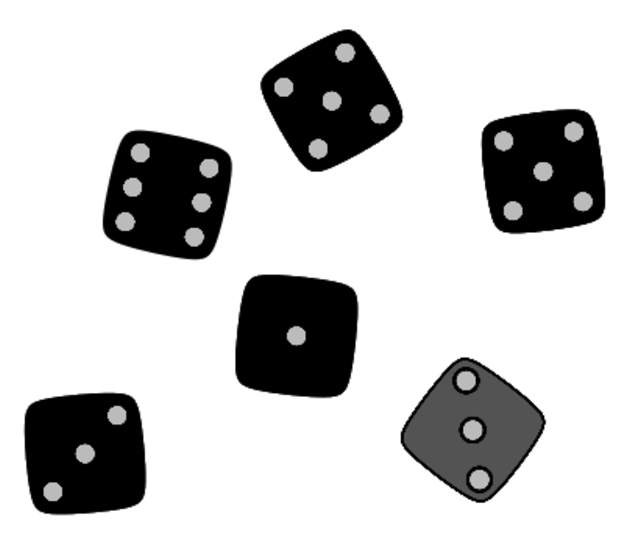
\includegraphics[scale=0.5]{Figs/Combinatorics/throw}
\end{figure}
